% \documentclass{report}
% 
% \usepackage{fancyhdr}
\usepackage{fourier-orns}
\usepackage{hyperref}%% To refrence links / jumps
\usepackage{chngcntr} %% For some extra counters numberings
\usepackage[a4paper, right = 0.5in, left = 0.5in,top = 1in , bottom = 1in]{geometry}
\usepackage{etoolbox} %% Provides like a language for advanced customization
\usepackage{datetime} %% For dates of course
\usepackage{lastpage} %% provides pages numbers
\usepackage[sc]{titlesec} %% modify titles
\usepackage{enumerate}
\usepackage{cancel}
\usepackage{tikzsymbols}
\usepackage[dvipsnames]{xcolor}
\usepackage{import}
\usepackage{pdfpages} %% include other pdfs
\usepackage{transparent} %% Transparency
\usepackage{xcolor}  %% Colors
\usepackage[many]{tcolorbox}
\usepackage[framemethod=TikZ]{mdframed}
\usepackage{amsmath,amsfonts,amsthm,amssymb,mathtools}
\usepackage{tikz}
\usepackage{bookmark}
\usepackage{graphicx}
\usepackage{mathpazo}

\usepackage{fontawesome5}

\linespread{1.5}


\titleformat{\chapter}[display]   
{\fontfamily{ppl}\selectfont\huge\color{YellowOrange!80!orange}} % Font style and size 
{\raggedleft\color{purple}\fontsize{70}{0pt}\selectfont\thechapter}   
{-1.5cm}    			                          % Space between the chapter number and title
{
	\begin{tikzpicture}[overlay]
		\node[anchor = west,yshift = 0.2cm,xshift = -1cm] {\fontsize{90}{20} $\int_{}^{} $};
		\node[yshift = 4cm, xshift = 17cm]   {\includegraphics[width = 4cm]{preview0}};
	\end{tikzpicture}
\hspace{1cm}\Huge\raggedright\MakeUppercase}

\titleformat{\section}[block]
{
\fontfamily{ppl}\selectfont\huge\color{YellowOrange!80!orange}
}
{
\color{purple}\fontsize{20}{0pt}\selectfont\thesection 
}
{0cm}
{
	\begin{tikzpicture}[overlay]
		\node[anchor = west,yshift = 0.2cm,xshift = -0.4cm, circle = 1pt] {};
	\end{tikzpicture}
}

\titlespacing*{\section}{0pt}{0.7cm}{1.5cm}


\newcommand{\divider}
{
	\begin{center}
	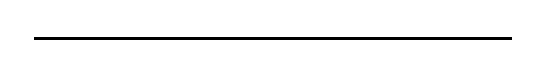
\begin{tikzpicture}
		\draw[thick, black] (0.25*\textwidth, 0) -- (0.75*\textwidth, 0);
		\node[rotate = 360 - 90, xshift = -0.6pt, yshift = 1pt] at (0.25*\textwidth,0){\decotwo};
		\node[rotate = 90, xshift = -0.6pt, yshift = 1pt] at (0.75*\textwidth,0){\decotwo};
	\end{tikzpicture}
	\end{center}
}

\pagestyle{fancy}

\newcommand{\lecday}[1][]
{
    \def\datee{#1}
    \fancyhead[L]{\datee}
}



\newcommand{\signature}
{
	\begin{tikzpicture}[remember picture,overlay]
		\node[fill = YellowOrange!20!white] at ([yshift = 1cm, xshift = -3cm]current page.south east) {\fontsize{10pt}{0pt}{\itshape Kara.$\mathcal{A}$}};
	\end{tikzpicture}
}

\AddToHook{shipout/background}{
  \begin{tikzpicture}[remember picture, overlay]
	  \node[] at ([yshift = 1.5cm,xshift = \textwidth /2 + 0.9cm]current page.south west) {\includegraphics[width = 0.5cm]{preview3}};
	  \node[] at ([yshift = 1.5cm,xshift = - \textwidth /2 - 0.9cm]current page.south east) {\includegraphics[width = 0.5cm]{preview4}};
  \end{tikzpicture}
}



\newtcolorbox[auto counter, number within = section]{remark}[1][]
{
       		title = Remark #1,
		enhanced,
		boxrule = 0pt,
		colback = white,
		breakable,
		arc = 4pt,
		colbacktitle = cyan,
		colback = cyan!5!white,
		segmentation style =
		{
			solid,cyan,thick,
		},
		attach boxed title to top left =
		{
			xshift = 0cm,
		},
		boxed title style =
		{
			boxrule = 0pt,
			sharp corners,
			drop fuzzy shadow = {cyan},
		},
		drop fuzzy shadow = {cyan!80!black},
}

\newtcolorbox[auto counter, number within = section]{theorem}[1][]
{                                      
		title = Theorem \thetcbcounter : #1,
		enhanced, 
		boxrule = 0pt,
		colback = white,
		breakable,
		arc = 4pt,
		colbacktitle = purple,
		colback = purple!5!white,
		segmentation style = 
		{
			solid, purple,thick,
		},
		attach boxed title to top left = 
		{
			xshift = 0cm, 
		},
		boxed title style = 
		{
			boxrule = 0pt,
			sharp corners,
			drop fuzzy shadow = {purple},
		},
		drop fuzzy shadow = {purple!80!black},
}

\newtcolorbox[auto counter, number within = section]{definition}[1][]
{                                      
		title = Definition \thetcbcounter : #1,
		enhanced, 
		boxrule = 0pt,
		colback = white,
		arc = 4pt,
		breakable,
		colbacktitle = YellowOrange!80!black,
		segmentation style = 
		{
			solid, YellowOrange,thick,
		},
		attach boxed title to top left = 
		{
			xshift = 0cm, 
		},
		colback = YellowOrange!5!white,
		boxed title style = 
		{
			boxrule = 0pt,
			sharp corners,
			drop fuzzy shadow = {YellowOrange!80!orange},
		},
		drop fuzzy shadow = {YellowOrange!80!black},
}

\newtcolorbox[auto counter, number within = section]{corollary}[1][]
{                                      
		title = corollary \thetcbcounter : #1,
		enhanced, 
		boxrule = 0pt,
		colback = white,
		arc = 4pt,
		breakable,
		colbacktitle = YellowOrange!80!black,
		segmentation style = 
		{
			solid, YellowOrange,thick,
		},
		attach boxed title to top left = 
		{
			xshift = 0cm, 
		},
		colback = YellowOrange!5!white,
		boxed title style = 
		{
			boxrule = 0pt,
			sharp corners,
			drop fuzzy shadow = {YellowOrange!80!orange},
		},
		drop fuzzy shadow = {YellowOrange!80!black},
}


\newtcolorbox{example}[1][]
{                                      
		title = Example,
		enhanced, 
		boxrule = 0pt,
		colback = white,
		arc = 4pt,
		segmentation style = 
		{
			solid, SpringGreen,thick,
		},
		breakable,
		colback = SpringGreen!5!white,
		colbacktitle = SpringGreen!80!black,
		attach boxed title to top left = 
		{
			xshift = 0cm, 
		},
		boxed title style = 
		{
			boxrule = 0pt,
			sharp corners,
			drop fuzzy shadow = {SpringGreen!80!orange},
		},
		drop fuzzy shadow = {SpringGreen!80!black},
}


\newcommand{\integral}[4]{\int\limits_{#1}^{#2} #4 d#3}
\newcommand{\limit}[3]{\lim\limits_{#1 \rightarrow #2} #3}
\newcommand{\strone}[2]{\left[ \begin{gathered}#1\\ #2\end{gathered} \right] }
\newcommand{\strtwo}[2]{\left\{ \begin{gathered}#1\\ #2\end{gathered} \right\} }
\newcommand{\strthree}[2]{\left\lfloor \begin{gathered}#1\\ #2\end{gathered} \right\rfloor }


\newcommand{\startbf}[1]{\text{\bfseries{#1}}}
\newcommand{\sett}[1]{\left\{ #1 \right\}}
\newcommand{\thesis}[1]{\left( #1 \right)}
\newcommand{\brkt}[1]{\left[ #1 \right]}
\newcommand{\floor}[1]{\left\lfloor #1 \right\rfloor}


\DeclareMathOperator{\img}{im} % Image
\DeclareMathOperator{\Img}{Im} % Image
\DeclareMathOperator{\coker}{coker} % Cokernel
\DeclareMathOperator{\Coker}{Coker} % Cokernel
\DeclareMathOperator{\Ker}{Ker} % Kernel
\DeclareMathOperator{\rank}{rank}
\DeclareMathOperator{\Spec}{Spec} % spectrum
\DeclareMathOperator{\Tr}{Tr} % trace
\DeclareMathOperator{\pr}{pr} % projection
\DeclareMathOperator{\ext}{ext} % extension
\DeclareMathOperator{\pred}{pred} % predecessor
\DeclareMathOperator{\dom}{dom} % domain
\DeclareMathOperator{\ran}{ran} % range
\DeclareMathOperator{\Hom}{Hom} % homomorphism
\DeclareMathOperator{\Mor}{Mor} % morphisms
\DeclareMathOperator{\End}{End} % endomorphism


\newcommand{\lm}{\ensuremath{\lambda}}
\newcommand{\eps}{\ensuremath{\epsilon}}
\newcommand{\veps}{\ensuremath{\varepsilon}}
\newcommand{\al}{\ensuremath{\alpha}}
\newcommand{\bb}{\ensuremath{\beta}}
\newcommand{\cc}{\ensuremath{\gamma}}
\newcommand{\dd}{\ensuremath{\delta}}
\newcommand{\DD}{\ensuremath{\Delta}}
\newcommand{\ff}{\ensuremath{\phi}}
\newcommand{\FF}{\ensuremath{\varphi}}

\newcommand{\RR}{\mathbb{R}}
\newcommand{\RO}{\mathcal{R}}
\newcommand{\EE}{\mathbb{E}}
\newcommand{\CC}{\mathbb{C}}
\newcommand{\RW}{\mathbb{R}^2}
\newcommand{\RT}{\mathbb{R}^3}
\newcommand{\RN}{\mathbb{R}^n}
\newcommand{\DS}{\mathcal{D}}

\newcommand{\KK}{\mathbb{K}}
\newcommand{\KW}{\mathbb{K}^2}
\newcommand{\KT}{\mathbb{K}^3}
\newcommand{\KN}{\mathbb{K}^n}

\newcommand{\NN}{\mathbb{N}}

\newcommand{\PS}{\mathcal{P}}
\newcommand{\AS}{\mathcal{E}}
\newcommand{\FS}{\mathcal{F}}
\newcommand{\LS}{\mathcal{L}}
\newcommand{\MS}{\mathcal{M}}

















% 
\lecday[2025-04-22]

% \begin{document}

\begin{theorem}[(The closed graph theorem)]
	Let $E $ and $F $ be two Banach spaces
	over some field $\KK = \RR  $ or $\CC  $ and 
	$ f : E \longrightarrow F $ be a linear mapping, 
	then $f $ is continuous if and onyl if its graph
	$G(f)  $  is closed in the Banach space 
	$E \times F  $, Recall that 
	\[
	G(f) := 
	\left\{ (x, f(x) ) : x \in  E \right\}
	\]
\end{theorem}
\begin{proof}
\[
	( \implies ) 
\]
Suppose that $f $ is continuous and show that 
$G(f)  $  is closed in $E \times F  $. So, let 
$\left\{ (x_{n}, f(x_{n}) )  \right\}_{n \in \NN} $, be an 
arbitrary sequence of $G(f)  $, converging in $E \times F  $ 
to some $(x,y) \in  E\times F  $ and let show that  
\[
	(x,y)  \in  G(f)  \quad y = f(x) 
\]
since the projections are continuous 
\[
\begin{array}{cccc}
      \pi _{1} : & E \times F    & \longrightarrow &  E\\

           &    (u,v) & \longmapsto     &  u\\ 
\end{array}
\]
and 
\[
\begin{array}{cccc}
      \pi _{2} : &  E \times F   & \longrightarrow &  F\\

           &    (u,v) & \longmapsto     &  v\\ 
\end{array}
\]
are both continuous, then the fact 
\[
	(x_{n}, f(x_{n}) )  \rightarrow (x,y) \quad 
	\text{ as } \quad n \rightarrow \infty 
\]
implies 
\[
	x_{n}  \rightarrow x \quad 
	f(x_{n})  \rightarrow y  \quad \text{ as } \quad 
	n \rightarrow \infty 
\]
But on the other hand, we have 
since $f $ is continuous, we have 
\[
x_{n} \rightarrow  x \text{ (in E) }  \implies 
f(x_{n})  \rightarrow  f(x)  \text{ (in F) } \quad \text{ as } n \rightarrow \infty  
\]
It follows according to the uniqueness of the limit that $y = f(x)  $,
as required.
\[
	(  \impliedby ) 
\]
Conversly, suppose that $G(f)  $  is closed in $E \times F  $.
This implies that the vector subspace 
$G(f)  $  of $E \times F  $  is Banach (a closed susbet of
complete space is complete). Next, consider the two maps, 
\[
p_1 = \pi _{1|_{G(f) }} \quad 
p_2 = \pi _{2|_{G(f) }}
\]
where
\[
\begin{array}{cccc}
      p_1 : &  G(f)   & \longrightarrow & E \\

           &  (u,f(u) )   & \longmapsto     & u \\ 
\end{array}
\]
and 
\[
\begin{array}{cccc}
      p_2 : &  G(f)   & \longrightarrow & F \\

           &  (u,f(u) )   & \longmapsto     & f(u)  \\ 
\end{array}
\]
Since $\pi _{1} $ and $\pi _{2} $ 
are linear and continiuous then $p_1 $ and $p_2 $ are 
also linear and continuous, Besides $p_1 $ is clearly
bejictive. So according to the Banach Isomorphism 
theorem we get that $p_{1}^{-1} $  is continuous, then,
\[
\begin{array}{cccccc}
	f : &  E  & \longrightarrow & G(f) &\longrightarrow & F  \\
	    &    u& \longmapsto     &  (u,f(u) )&\longrightarrow & f(u)\\ 
\end{array}
\]
clearly 
\[
f = p_{2} \circ  p_1^{-1}
\]

is continuous, since its a composition of two continuous maps,
as required. this completes the proof of the theorem.
\end{proof}
\begin{center}
	\it The Banach-Steinhans Theorem \normalfont
\end{center}
\begin{definition}[Meager Sets]
	Let $E $ be a toplogical space and $X $ be 
	a subset of $E $. Then $X $ is said to
	be meager if it can be included in a countable
	union of closed subsets of $E $ of empty interior. \\
	Equivalently, $X $ is meager if its a countable union of 
	subsets whose closure has empty interior.
\end{definition}
A set that is not meager is said to be nonmeager 
\begin{example}
\begin{enumerate}
\item $Q $ is meager in $\RR  $ equipped with its usual toplogy.
	Indeed we can write, 
	\[
	Q = \bigcup_{n \in Q}^{}  \left\{ n \right\}
	\]
	$\left\{ x \right\} $  is closed in $\RR  $, and 
	$\mathring{\overline{\left\{ x \right\}}} = \emptyset $, 
	Other method is, 
	\[
	Q = \mathbb{Z} \cup  \frac{1}{2} \mathbb{Z} \cup 
	\frac{1}{3} \mathbb{Z} \cup  \hdots 
	\]
	for all $n \in  \NN $, we have 
	\[
		\mathring{\overline{\frac{1}{n}\mathbb{Z}}} = 
		\frac{1}{n} \mathring{\overline{\mathbb{Z}}} = 
		\emptyset 
	\]
	since $\overline{\mathbb{Z}} = \mathbb{Z} $  and 
	$\mathring{Z} = \emptyset $ 
\item Let $E $ be Baire space (i.e., a toplogical space that satisfies
	the Baire property).  
	\begin{itemize}
		\item $E $ is nonmeager in $E$.
			\begin{proof}
				\it 
	Indeed if $E = \bigcup_{n=0}^{\infty } F_{n} $, where
	$F_{n} = \emptyset,  \forall n \in \NN $, then 
	since $E $ is Baire we get $\mathring{E}=  \emptyset  $, which
	is a contradiction \normalfont.
			\end{proof}
		\item More generally, if 
			$A$ is a meager subset of $E $, then 
			$E \backslash A $  is dense in $E$ 
		\begin{proof}
		Since $A $ is meager then we have 
		\[
		A \subset \bigcup_{n=1}^{\infty } F_{n} \quad 
		\mathring{F_{n}}= \emptyset  \quad 
		\forall n \in \NN 
		\]
		Since $E $ is Biare then 
		$\mathring{\bigcup_{n=1}^{\infty } F_{n}}=\emptyset  $.
		Thus $\mathring{A} \subset \mathring{\bigcup_{n=1}^{\infty } }
		=\emptyset $, thus $\mathring{A}=\emptyset  $, hence
		\[
			\overline{
			E \backslash A} = 
			E \backslash \mathring{A} = 
			E \backslash \emptyset = E
		\]
		that is $X \backslash A $  is dense in $E $ 
		\end{proof}
	\end{itemize}
\end{enumerate}
\end{example}
\begin{theorem}[Banach-Steinhaus 1927]
	Let $E $ and $F $ be two N.V.S for a family of
	continuous mappings 
	from $E $ to $F $ to be uniformally bounded on the unit
	ball of $E $, it sufficies that it be pointwise bounded on
	a noneager subset of $E$. 
\end{theorem}
\begin{definition}[(Uniformally bounded in Unit ball)]
	$(f_{i}) _{i \in I} $  linear continuous.
	\[
	\exists M > 0, \forall x \in  B_{E}(0_{E},1)  
	\| f_{i}(x)  \|  \leq M 
	\]
\end{definition}
\begin{definition}[(Pointwise bounded on A)]
	Pointwise bounded on $A$, for all $x \in  A $, 
	$\exists M_{x} $  such that,  
	\[
	\forall i \in  I : \quad 
	\| f_{i}(x)  \|  \leq M_{x}
	\]
\end{definition}
More explicitly, let $A \subset \mathcal{L} (E,F)  $, 
and for all $x \in  E $, let 
\[
A_{x} := \left\{ 
f(x) , f \in  A\right\}
\]
Finally, let 
\[
B :=  \left\{ x \in  E, A_{x} \text{ is bounded in } F  \right\}
\]                                                   
Suppose that $B$ is nonmeager in $E $, then 
$A $ is bounded in $\mathcal{L} (E,F)  $,
In particular $B = E $ 
\begin{proof}
We can write $B $ as, 
\begin{align*}
	B &= \bigcup_{n=1}^{\infty }  
	\left\{ x \in E, 
	A_{x} \text{ is bounded by $n $ in $F $ } \right\} \\
	  &= 
	  \bigcup_{n=1}^{\infty } 
	  \left\{ x \in E: \| f(x)  \| _{F} \leq n, 
	  \forall f \in  A\right\} 
\end{align*}
next for all $n \in \NN $, we have 
\[
B_{n} = \bigcap_{f \in  A}^{}  
\underbrace{
\left\{ x \in  E: \| f(x)  \| _{F} \leq n \right\}
}_{B_{n,f}} 
\]
since for any $n \in \NN$  and 
any $f \in  A $, $B_{n,f} $  is the preimage of the 
closed subset $(-\infty ,n]  $  of $\RR  $  by the 
continuous map
\[
\begin{array}{cccc}
        &  E  & \longrightarrow & \RR  \\

           &  x  & \longmapsto     & 
	   \| f(x)  \| = \|   \| \circ  f\\ 
\end{array}
\]
then $B_{n,f} $ is closed in $E $ for all
$n \in \NN, \forall f \in A$, thus 
$B_{n}(n \in \NN)  $  is closed in $E $ 
as its the intersction of closed subsets 
of $E $,but since $B $ is non meager and 
$B = \bigcup_{n=1}^{\infty } B_{n}  $ , where 
$B_{n} $ is closed for all $n $, there exist
$N \in \NN $  such that 
\[
\mathring{B_{N}} \neq \emptyset 
\]
therefore $\exists x_0 \in  E, 
\exists r > 0$  such that 
\[
B_{E}(x_0, r)  \subset B_{N}
\]
Now, for all $f \in  A $ and for all 
$x \in  B_{E}(0_{E},1)  $, we have that 
\[
x_0 (+/-) rx \in B_{E}(x_0,r) \subset B_{N} 
\]
implying that 
\[
\| f(x_0 (+/-) rx )  \| _{F} \leq N
\]
consequently, we have 
\[
\forall f \in  A, \forall x \in  B_{E}(0_{E},1)
\quad 
f(x) = f \left( \frac{1}{2r}[(x_0 +rx) - (x_0-rx) ] \right) 
\]
since $f $ is linear we get 

\[
f(x) = \frac{1}{2r} \left[ 
	f(x_0 + rx)  - f(x_0 -rx) 
\right]
\]
thus \[
\forall  f \in  A, \forall  x \in B_{E}(0_{E},1) 
\]
we get 
\begin{align*}
	\| f(x)  \| _{F} & \leq 
	\frac{1}{2r}
	\left[ \| f(x_0+rx)  \| _{F} + 
	\| f(x_0-rx)  \| _{F}\right] \\
			 & \leq  \frac{N}{r}
\end{align*}
implying that 
\[
\mid \mid \mid  f \mid \mid \mid \leq  \frac{N}{r}
\quad  ( f \in A) 
\]
showing that $A $ is bounded in $\mathcal{L} (E,F)  $,
as required.

\end{proof}


before we continue the main proof, we will add some
small theorems
\begin{theorem}[1]
	Let $E $ be a Banach space
	and $F $ be an arbitrary N.V.S. Let also
	$A $ be a subset of $\mathcal{L} (E,F)  $.
	Then the two following properties are equivalent, 
	\begin{enumerate}[(i)]
	\item $A $ is bounded in $\mathcal{L} (E,F)  $ 
	\item for all $ x \in E $, the subset 
		\[
		\left\{ f(x) , f \in A \right\} \text{ of } 
		F \text{ is bounded. } 
		\]
	\end{enumerate}
\end{theorem}
\begin{proof}
Since $E $ is Banach then its Baire, 
hence $E $ is nonmeager in it self
the result of the corollary then follows
from the previous proof.
\end{proof}
\begin{theorem}[2]
	Let $E $ be a Banach soace, and $F $ be 
	an arbitrary N.V.S. Let also
	$(f_{n}) _{n \in \NN} $  
	be a sequence of $\mathcal{L} (E,F)  $, 
	suppose that for all $x \in E $, the sequence
	$(f_{n}(x) )_{n \in \NN}  $  converges in $F $ 
	and denote by $f(x)  $  its limit, then 
	\begin{itemize}
	\item 
	$(f_{n})_{n \in \NN}   $  is bounded in 
	$\mathcal{L} (E,F)  $
	\item  
	$f \in  \mathcal{L} (E,F)  $ 
	\item  
	$\mid \mid \mid  f \mid \mid \mid \leq 
	\lim_{n \to \infty} inf \mid \mid \mid  f_{n} \mid \mid \mid $ 
	\end{itemize}
\end{theorem}
\begin{proof}
	\begin{center}
		The Boundedness of $f $ 
	\end{center}
	
	for all $x  \in E$, since the sequence 
	$(f_{n}) _{n \in \NN} $  of $F $ is assumed 
	convergent, then its bounded. this implies 
	implies according to the Theorem $1 $, that the sequence
	$(f_{n}) _{n \in \NN} $ of $\mathcal{L} (E,F) $  is 
	bounded.
	\begin{center}
		The Linearity of $f $ (obvious) 
	\end{center}
	for all $\lm \in  \KK $, $\forall x,y \in  E $, we have, 
	\begin{align*}
		f(\lm x + y)  &= 
		\lim_{n \to \infty} f_{n}(\lm x + y)   \\
			      &= \lim_{n \to \infty} 
			      \left( \lm f_{n}(x)  + 
			      f_{n}(y) \right) \\
			      &= \lm \lim_{n \to \infty} 
			      f_{n}(x)  + 
			      \lim_{n \to \infty} f_{n}(y)  \\
			      &= \lm f(x) + f(y) 
	\end{align*}
	showing that $f $ is linear.
	\begin{center}
		The continuity of $f $ and the estimate of 
		$\mid \mid \mid  f \mid \mid \mid  $,
	\end{center}
	$\forall x \in E $, we have 
	\begin{align*}
		\| f(x)  \| _{F} &= 
		\| \lim_{n \to \infty} f_{n}(x)  \| _{F} \\
				 &= 
				 \lim_{n \to \infty} 
				 \| f_{n}(x)  \| _{F} \\
				 &= 
				 \lim_{n \to \infty} inf 
				 \| f_{n}(x)  \| _{F} \\
				 & \leq 
				 \lim_{n \to \infty} inf 
				 \left( 
					 \mid \mid \mid  f_{n} \mid \mid \mid  
					 \| x \| _{E}
				 \right) = 
				 \left( \lim_{n \to \infty} inf
				 \mid \mid \mid  f_{n} \mid \mid \mid 
			 \right) \| x \| _{E}
				 \\ 
	\end{align*}
	implying that $f $ is continuous and that 
	\[
	\mid \mid \mid  f \mid \mid \mid  \leq \lim_{n \to \infty} inf
	\mid \mid \mid  f_{n} \mid \mid \mid 
	\]
	 This completes the proof.
\end{proof}
% (f _1, f_2, f_3, ...) in L(E,F) 
% if (f _1, f_2, f_3, ...)  satisfies
%    for all x in non eager set (A), 
%    there exist M_x such that 
%    || f_i(x) || <= M_x
%	=>
% ||| f ||| <= M in unit ball
%
%
%
%
%
% \end{document}
